\documentclass[a4paper,12pt]{book}

% Paquetes necesarios
\usepackage[utf8]{inputenc}   % Codificación de caracteres
\usepackage[spanish]{babel}   % Idioma español
\usepackage[T1]{fontenc}      % Codificación de fuentes
\usepackage{amsmath, amssymb} % Símbolos matemáticos
\usepackage{graphicx}         % Inclusión de gráficos
\usepackage{cite}             % Gestión de citas
\usepackage{hyperref}         % Enlaces y referencias
\usepackage{geometry}         % Configuración de márgenes
\usepackage{fancyhdr}         % Encabezados y pies de página
\usepackage{titlesec}         % Formato de títulos
\usepackage{booktabs}         % Tablas profesionales
\usepackage{caption}          % Personalización de leyendas
\usepackage{enumitem}         % Personalización de listas
\usepackage{float}
\usepackage{tcolorbox}
\usepackage[table]{xcolor} % Paquete para colores en tablas
\usepackage{colortbl}       % Complemento para colorear celdas específicas
\usepackage{multirow}       % Combinar celdas en tablas
\usepackage{makecell}       % Combinar celdas en tablas
\usepackage{enumitem}
\usepackage{amsmath}
\usepackage{eurosym}
\usepackage{tikz}
\usepackage{listings}
\usepackage{color}
\usepackage{float}
\usepackage{pdfpages}

% Configuración de márgenes
\geometry{left=3cm, right=3cm, top=2.5cm, bottom=2.5cm}

% Configuración de encabezados y pies de página
% \setlength{\headheight}{14.49998pt}
\pagestyle{fancy}
\fancyhf{}

\fancyhead[L]{Universidad de Granada}
\fancyhead[L]{\nouppercase{\chaptername~\thechapter. \leftmark}}

% \fancyhead[C]{Escuela Técnica Superior de Ingenierías Informática}

%\fancyhead[L]{Universidad de Granada}
\fancyhead[L]{\nouppercase{\leftmark}}
\fancyhead[R]{Inteligencia Artificial}
\fancyfoot[L]{\rule[0pt]{\textwidth}{0.2pt}\\Ismael Sallami Moreno}
\fancyfoot[C]{\rule[0pt]{\textwidth}{0.2pt}\\\thepage}
\fancyfoot[R]{\rule[0pt]{\textwidth}{0.2pt}\\\today}


\renewcommand{\sectionmark}[1]{\markboth{#1}{}} % Configura \leftmark para que solo muestre la sección


% Formato de títulos
\titleformat{\section}{\large\bfseries}{\thesection.}{0.5em}{}
\titleformat{\subsection}{\normalsize\bfseries}{\thesubsection.}{0.5em}{}

% Datos del documento
\title{\textbf{Temario Inteligencia Artificial}}
\author{
    Ismael Sallami Moreno \\
    \texttt{ism350zsallami@correo.ugr.es}
}
\date{
    \vspace{1cm}
    \begin{tabular}{rl}
        \textbf{Asignatura:} & Inteligencia Artificial \\
        \textbf{Tema:} & Temario \\
        \textbf{Fecha:} & \today
    \end{tabular}
}

\begin{document}

% Portada
\begin{titlepage}
    \begin{center}
        % \vspace*{1cm}
        
        % \Huge
        % \textbf{Práctica Contabilidad Financiera II}
        \Huge \textbf{Temario Inteligencia Artificial} 
        % \vspace{0.5cm}
        % \LARGE
        % \textbf{Ismael Sallami Moreno}\\
        % \LARGE
        % \texttt{ism350zsallami@correo.ugr.es}
        % \LARGE
        % \url{https://github.com/Ismael-Sallami}
        
        % \vfill
        
        % \Large
        % \textbf{Universidad de Granada}
        
        \vspace{0.8cm}
        
        \begin{tikzpicture}[remember picture, overlay]
            \node[opacity=0.2] at (current page.center) {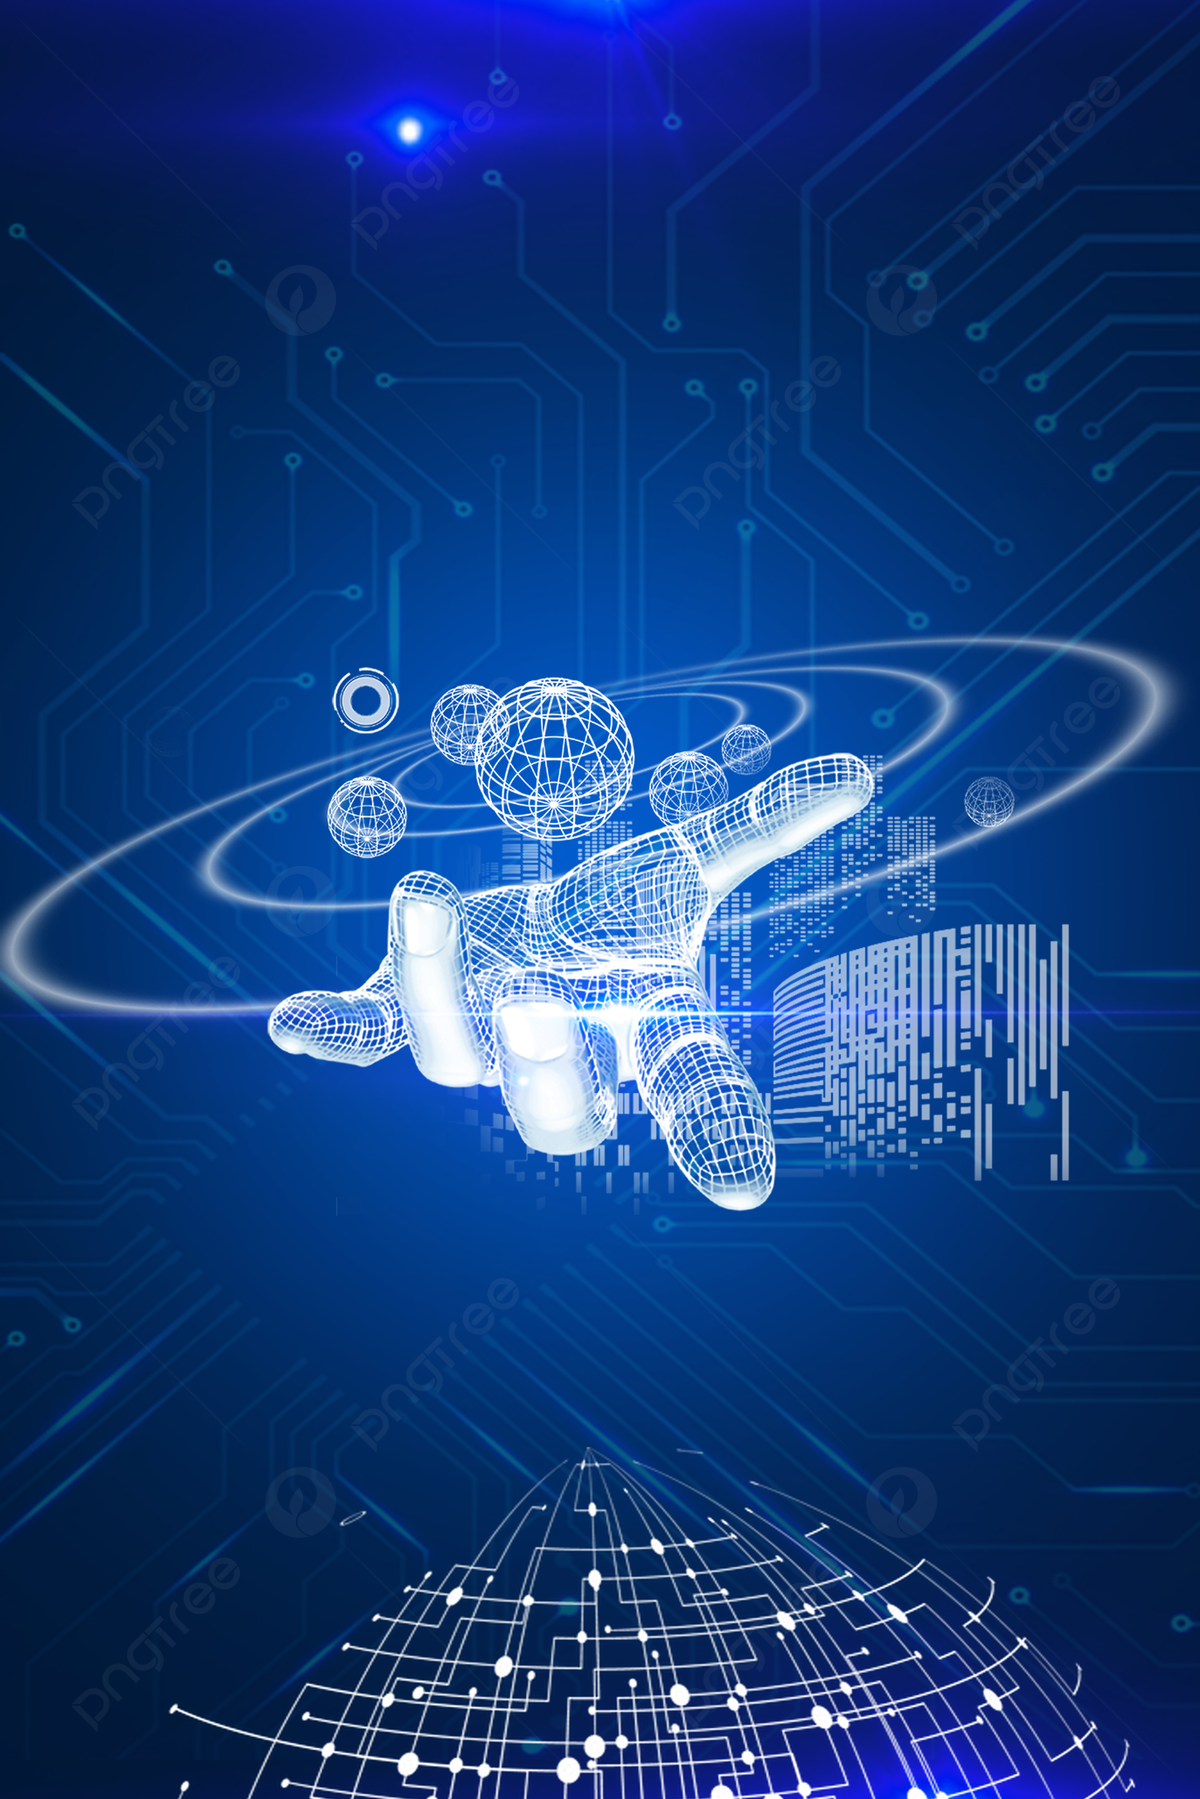
\includegraphics[width=\paperwidth,height=\paperheight]{portada.png}};
            \node[align=center] at (current page.center) {
                
                \vspace{0.5cm}
                \LARGE \textbf{Ismael Sallami Moreno} \\
                \LARGE \texttt{ism350zsallami@correo.ugr.es} \\
                \LARGE \url{https://ismael-sallami.github.io/} \\
                \LARGE \url{https://elblogdeismael.github.io/} \\
                \vspace{2cm}
                \Large \textbf{Universidad de Granada} \\
                \vspace{0.8cm}
                % \Large \textbf{2025}
            };
        \end{tikzpicture}
        \vfill
        
        \Large
        \textbf{2025}
        
    \end{center}
\end{titlepage}
\newpage


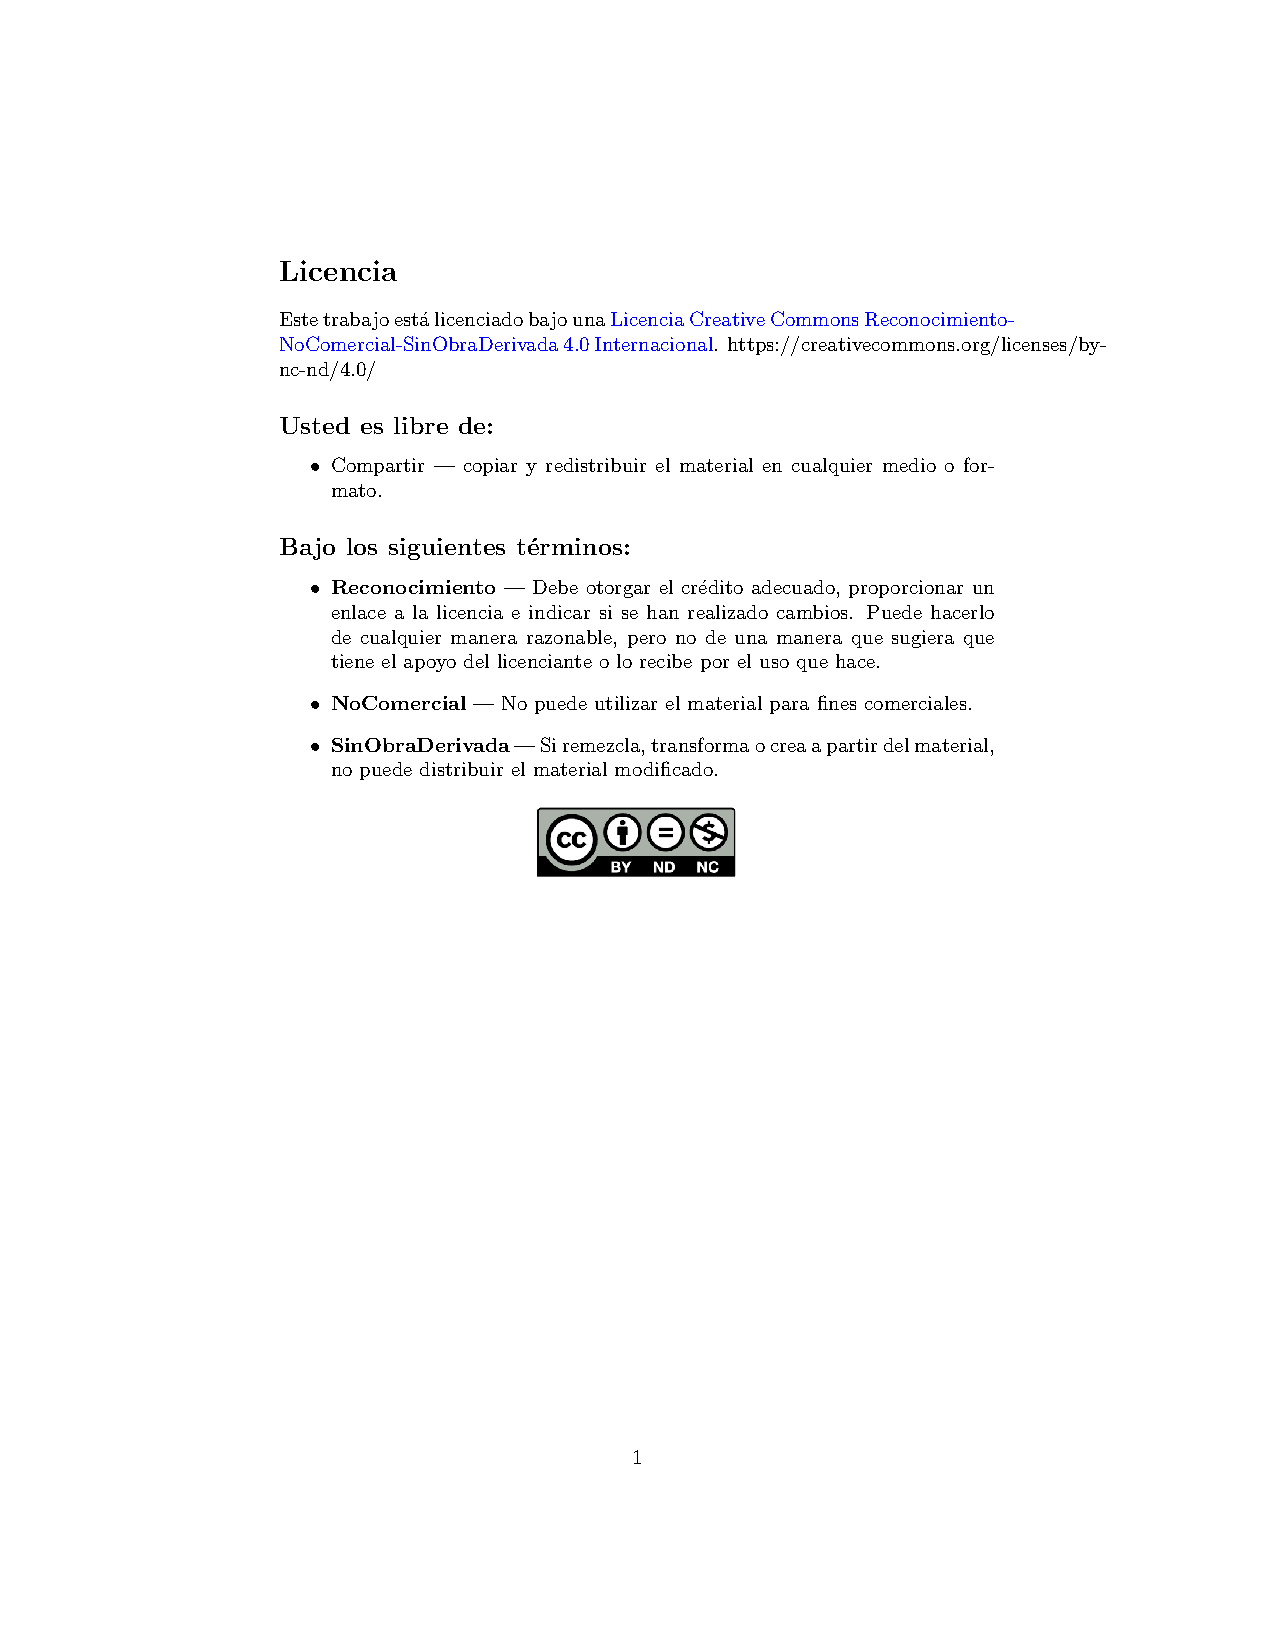
\includepdf[pages=-]{../../../../licencia.pdf}

% Tabla de contenidos
\tableofcontents
\newpage

% \chapter{Introducción}
% \section{Apuntes de CLase}
% \section{Introducción: Inteligente}
Debemos de definir la inteligencia artificial
usando la palabra inteligente, la cual es difícil de definir. Se dan diferentes definiciones de Harvard y otras universidades/entidades reconocidas. 

\section{Definición de IA}

Podemos tener varias definiciones de IA, como pueden ser sistemas que actúan/piensan como humanos, o bien sistemas que actúan/piensas racionalmente. Una de ellas puede ser: "Campo de estudio que busca explicar y emular el comportamiento inteligente en términos de procesos computacionales"

Un ejemplo de IA que menciona el profesor reiteradamente es el caso de los \textit{cajeros automáticos}.

\begin{tcolorbox}[colback=blue!20, colframe=blue]
Se garantiza que una pregunta sobre las definiciones de IA cae.
    
\end{tcolorbox}

Asociamos el concepto de IA a racional debido a que se quiere desarrollar con la capacidad de poder tomar decisiones como los humanos.

Hay distintos softwares en los dispositivos que podemos relacionarlos con la acción de que \textit{piensan} debido a que usan inteligencia artifical, como es el caso de programas de ajedrez. ¿Es esto correcto? No podemos afirmar esto exactamente, ya que según autores pensar es emular la mente humana, cosa que no es capaz de hacer la IA debido a que solo esta entrenado a hacer las mejores jugadas para ganarte, mientras que tu puedes pensar sobre otras temáticas y tener cierto \textit{pensamiento libre}.

Si afirmamos que piensan como humanos, debemos de tener en cuenta el \textit{pensamiento cognitivo}.

La IA según el libro del \textit{Porque} (recibió el premio Turing), tiene 3 niveles:
\begin{enumerate}
    \item Aprendizaje automático.
    \item Simular al humano.
    \item Capacidad de imaginar, lo cual, a día de hoy es inalcanzable.
\end{enumerate}

En cuanto a la creatividad, hay cierta\textit{ creatividad cognitiva }en temas específicos.

El llamado 'no alineamiento con los humanos' es lo que ocurre cuando una IA no tiene información sobre ese tema o bien no esta entrenado, pues en este caso se lo inventa.

El Test de Turing, es aquel en el que si una IA consigue pasar desapercibido como humano, pues efectivamente pasa este Test.

En esta asignatura vamos a seguir la Teoría del Agente, que es la idea más aceptada hoy día y más usada. Este percibe el entorno y actúa de una manera específica. 

Se usa la palabra \textit{racional} aludiendo a inteligente.

Un agente racional actúa de manera correcta según la información que posee.

El origen del término de IA recae en John McCarthy. Los pioneros de la IA son varios, entre los que podemos encontrar a Alan Turing, Marvin Minsky,...

En el debate de la IA se menciona una IA fuerte y una débil, que son sistemas que actúan como humanos y racionalmente vs las que piensan como IA.

En cuanto al recorrido de la IA a lo largo de la historia, podemos destacar distintas épocas como es la Edad de Oro, Invierno de IA,...

Von Neumann propone el algoritmo MiniMax, el que afirma que el juego es una situación conflictiva en la que tomamos decisiones sabiendo que los demás también las toman, determinando el resultado en base a las decisiones realizadas.
Un hecho histórico destacable, es que Napoleón murió pensando que había perdido jugando al ajedrez pensando que perdió frente al primer sistema inteligente, aunque puede que haya sido un humano. 
Otro de los avances importantes es el caso de los cohes autónomos.

En cuanto a los tipos de IA podemos mencionar:

\begin{itemize}
    \item IA débil: una máquina que compite con un humano en una actividad específica.
    \item IA fuerte: IA que aplica inteligencia para cualquier problema.
    \item IA general: alcanza el nivel cognitivo humano.
    \item Super-IA: capacidad que es mucho mayor que cualquier cerebro humano en cualquier campo.
\end{itemize}


\chapter{Agentes}
% \section{Apuntes de CLase}
% \section{Concepto}
La Teoría de Agentes(denotado a continuación como \textbf{TA}) es un sistema de ordenador, situado en un entorno, capaz de realizar acciones de manera autónoma y que es flexible en base a las situaciones que se le presentan.

\section{Agentes Inteligentes}

Desarrolla un enfoque basado en agentes y lleva a cabo percepciones procesada mediante algoritmos de análisis y toma de decisiones. 
La TA se usa actualmente en la mayoría de ámbitos y es lo que más se usa hoy en día.

En cuanto a los tipos de agentes encontramos:

\begin{itemize}
    \item Reactivo: reacciona en base al entorno.
    \item Pro-activo: no solo actúan en respuesta al entorno, sino que puedan analizar acciones a llevar a cabo.
    \item  Social: son además capaces de interactuar.
    \item Multiagente: esta implementado como varios agentes interactuando.
\end{itemize}

La interacción entre agentes se lleva a cabo mediante: cooperación, coordinación y la negociación.


\section{Arquitecturas de Agentes}

Podemos distinguir entre:

\begin{itemize}
    \item Reactivo: reacciona en base a la situación en la que se encuentra, eligiendo la más adecuada en base a lo que sabe.
    \item Deliberativo: toma decisiones basadas en razonamiento, planificación y modelos internos del mundo.
\end{itemize}
\section{Relacion de Problemas 1}
\begin{tcolorbox}[colback=green!5!white, colframe=green!75!black]
\textit{Esta relación no suele caer en el examen, la 2 y la 3 sí.}
\end{tcolorbox}

\textbf{Podemos ver los códigos de los ejercicios 1,3,4 en el apartado de Asignaturas/Tercer Año/IA/Teoria/Capitulos/Elementos\_Relacion\_1 en la web del blog de ismael.}

\subsection*{Ejercicio 1}

Una hormiga artificial vive en un mundo bidimensional cuadriculado y desarrolla un 
comportamiento  que  le  permite  seguir  un  rastro  de  feromonas  a  lo  largo  de  un  conjunto  de 
casillas  previamente  marcadas  (el  tamaño  del  rastro  es  de  una  casilla).  La  hormiga  ocupa  una 
sola casilla y puede encarar las casillas que se encuentran arriba, a la derecha, a la izquierda y 
debajo  de  la  posición  en  la  que  se  encuentra.  La  hormiga  puede  llevar  a  cabo  tres  acciones: 
moverse a una celda hacia adelante (actFORWARD), girar a la izquierda permaneciendo en la 
misma casilla (actTURN\_L) y girar a la derecha permaneciendo en la misma casilla 
(actTURN\_R).  La  hormiga  puede  percibir  si  la  casilla  que  tiene  delante  (en  el  sentido  del 
movimiento) tiene feromona.

\begin{enumerate}
    \item Especificar  un  sistema  de  reglas  para  controlar  el  comportamiento  de  la  hormiga  en  el 
    seguimiento del rastro de la feromona. Suponer inicialmente a la hormiga en una casilla en 
    la que puede percibir el rastro de feromona.
    \item Resuelva el problema anterior con la siguiente restricción: la hormiga, una vez que llega a 
    una nueva casilla, no puede girar más de 180 grados desde la posición inicial.
\end{enumerate}

\subsubsection*{Solución}
Debemos de tener en cuenta las características de los agentes reactivos:
\begin{itemize}
    \item Sensores:
    \begin{itemize}
        \item Feromona: booleano.
    \end{itemize}
    \item Acciones.
    \begin{itemize}
        \item actFORWARD.
        \item actTURN\_L.
        \item actTURN\_R.
    \end{itemize}
    \item Reglas.
    \begin{itemize}
        \item Si percibo feronomonas delante de mi $\rightarrow$ actFORWARD y he\_girado\_Derecha = false.
        \item Si no feromona y no he\_girado\_Derecha $\rightarrow$ actTURN\_R y he\_girado\_Derecha = true.
        \item Si no feromona y he\_girado\_Derecha $\rightarrow$ actTURN\_L.
        % \item Si no (else) percibo feronomonas delante de mi, actTURN\_L o actTURN\_R (dependiento del que sea más conveniente).
    \end{itemize}
    \item Variables de estado.
    \begin{itemize}
        \item He\_girado\_Derecha (booleano). Se debe de inicializar a falso.
    \end{itemize}
\end{itemize}

Con esto tenemos definido completamente nuestro agente.

\subsubsection*{Anotaciones sobre el desarrollo del ejercicio}
\begin{itemize}
    \item Vemos que nuestra solución tiene fallos debido a que siempre esta girando hacia la derecha, así que debemos de hacer uso de las variables de estado para solucionar este problema.
    \item Tenemos el problema de que si se cruzan los caminos no pasará por uno de ellos.
\end{itemize}


\subsection*{Ejercicio 2}

La avispa hembra del género Sphex, deja sus huevos dentro de un grillo que ha paralizado y ha 
llevado  a  su  nido.  Las  larvas  de  la  avispa  salen  del  grillo  y  se  alimentan  de  él.  La  avispa 
presenta el siguiente comportamiento: lleva el grillo paralizado a su nido, lo deja en el umbral 
del nido, entra dentro del nido para ver si todo está correcto, sale, y entonces arrastra al grillo 
hacia  su  interior.  Si  el  grillo  se  mueve  cuando  la  avispa  está  en  el  interior  haciendo  la 
inspección preliminar, la avispa saldrá del nido, volverá a colocar el grillo en el umbral, pero no 
dentro, y repetirá el procedimiento de entrar en el nido para ver si todo está correcto. Si el grillo 
se mueve otra vez mientras la avispa está dentro del nido, ésta volverá a salir y colocar el grillo 
en  el  umbral,  entrando  de  nuevo  en  el  nido  para  realizar  la  inspección  preliminar.  En  una 
ocasión,  este  procedimiento  se  repitió  cuarenta  veces.  Define  características  y  acciones  para 
diseñar un agente reactivo que se corresponda con el comportamiento de la avispa.

\subsubsection*{Solución}

\begin{itemize}
    \item Sensores.
    \begin{itemize}
        \item Grillo\_movido: booleano.
    \end{itemize}
    \item Acciones.
    \begin{itemize}
        \item actLlevar\_Nido.
        \item actDejar\_Umbral.
        \item actEntrar\_Nido.
        \item actSalir\_Nido.
    \end{itemize}
    \item Reglas.
    \begin{itemize}
        \item Si grillo\_movido, actDejar\_Umbral.
        \item Si no grillo\_movido, actEntrar\_Nido.
    \end{itemize}
    \item Variables de estado.
    \begin{itemize}
        \item Grillo\_movido: booleano. Se debe de inicializar a falso.
    \end{itemize}
\end{itemize}   

\subsection*{Ejercicio 3}

Supongamos  que  un  agente  trabaja  sobre  un  tablero  formado  por  NxN  casillas.  Sobre  este 
tablero se definen dos zonas: una "zona interior" formada por un tablero de (N-2)x(N-2) casillas 
inscrito  en  el  tablero  general,  y  una  "zona  exterior"  formada  por  el  resto  de  las  casillas. Separando ambas zonas aparece una línea gruesa negra denominada "Frontera". En la figura se 
muestra un ejemplo de la configuración de un tablero 7x7. 
El  cometido  del  robot  consiste  en  llevar  todos  los  obstáculos  que  se  encuentren  en  la  zona 
interior a la zona exterior. El robot siempre se debe encontrar en la 
zona interior, y no debe nunca traspasar la frontera. 
Para  realizar  esta  tarea,  el  robot  dispone  de  3  sensores,  un  sensor 
de  choque  "BUMPER"  que  le  permite  detectar  el  obstáculo,  un 
sensor de infrarrojos "CNY70" que permite ver dónde está la línea 
de  la  Frontera,  y  una  brújula  digital  "Brujula"  que  le  indica  su 
orientación en el avance. Los dos primeros sensores se encuentran 
situados  en  la  parte  frontal  del  robot.  La  brújula  sólo  devuelve  4 
valores: 0, 1, 2 y 3, representando respectivamente Norte, Este, Sur 
y Oeste. 
 
Las acciones que puede realizar el robot son las siguientes: 
\begin{enumerate}
    \item Avanzar: Avanza una casilla en la dirección que marca su brújula siempre que no tenga 
    un obstáculo delante. 
    \item Retroceder:  Retrocede  una  casilla  en  la  dirección  contraria  a  la  que  indica  su  brújula, 
    siempre que no tenga un obstáculo detrás. 
    \item GirarI: Gira sin moverse de la casilla hacía la izquierda. 
    \item GirarD: Gira sin moverse de la casilla hacía la derecha. 
    \item Nada: No realiza ninguna acción 
    \item Empujar: Avanza una casilla en la dirección que marca su brújula. Para que está acción 
    tenga efecto, debe estar activado el sensor de choque. 
\end{enumerate}

Se pide: 
\begin{itemize}
    \item[a)] Definir  las  variables  de  estado  (nombre  e  descripción)  y  las  reglas  de  producción 
    necesarias  para  diseñar  un  agente  reactivo  con  memoria  que  partiendo  de  una  casilla 
    desconocida dentro de la zona interior de un tablero de dimensiones también 
    desconocidas (nunca superiores a 99x99), sea capaz de calcular la dimensión de la zona 
    interior, suponiendo que en el tablero no hay obstáculos. 
    \item [b)] Definir  las  variables  de  estado  y  las  reglas  de  producción  necesarias  que  permitan  al 
    robot localizar el obstáculo en el tablero. 
    \item [c)] Suponiendo  que  el  robot  se  encuentra  orientado  hacía  el  obstáculo  en  una  casilla 
    adyacente (es decir, el sensor BUMPER está activado) y que el obstáculo se encuentra 
    en  una  casilla  interna  del  tablero  que  no  es  adyacente  con  ninguna  casilla  pegada  a  la 
    frontera,  definir  las  variables  de  estado  y  las  reglas  de  producción  necesarias  que 
    permitan  al  robot  expulsar  el  obstáculo  hacía  la  zona  exterior,  arrastrándolo  por  el 
    camino más corto de casillas. 
\end{itemize}

\begin{figure}[H]
    \centering
    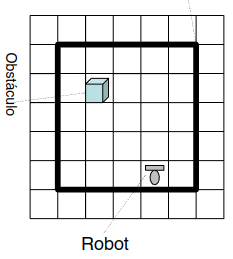
\includegraphics[width=0.35\textwidth]{images/ej3rel1.png}
    \caption{Imagen del tablero.}
    \label{fig:tablero}
\end{figure}

% \begin{figure}[h]
%     \centering
%     \begin{tikzpicture}
%         % Cuadrícula
%         \draw[step=0.5cm,gray,very thin] (0,0) grid (2.5,2.5);
        
%         % Borde del área negra
%         \draw[very thick] (0.5,0.5) rectangle (2,2);
        
%         % Obstáculo
%         \filldraw[gray!30] (1,1.75) rectangle (1.25,2);
%         \draw (1,1.75) rectangle (1.25,2);
        
%         % Robot
%         \filldraw[gray!30] (1.75,0.75) circle (0.2);
%         \draw (1.75,0.8) -- (1.75,0.65);
%         \draw (1.65,0.5) -- (1.85,0.5);
        
%         % Etiquetas
%         \node[rotate=90] at (-0.3,1.25) {Obstáculo};
%         \node at (1.25,-0.3) {Robot};
%     \end{tikzpicture}
%     \caption{Tablero con tikz.}
% \end{figure}


\subsubsection*{Solución a)}

\begin{itemize}
    \item Sensores.
    \begin{itemize}
        \item BUMPER: booleano.
        \item CNY70: booleano.
        \item Brujula: entero (0,1,2,3).
    \end{itemize}
    \item Acciones.
    \begin{itemize}
        \item Avanzar.
        \item Retroceder.
        \item GirarI.
        \item GirarD.
        \item Nada.
        \item Empujar.
    \end{itemize}
    \item Variables de estado.
    \begin{itemize}
        \item estoy\_contando: booleano. Se debe de inicializar a falso.
        \item estoy\_girando: booleano. Se debe de inicializar a falso.
        \item contador: entero. Se debe de inicializar a 0.
    \end{itemize}
    \item Reglas.
    \begin{itemize}
        \item Si no estoy\_contando y no estoy\_girando y no CNY70 $\rightarrow$ avanzar.
        \item Si no estoy\_contando y no estoy\_girando y CNY70 $\rightarrow$ girarI y estoy\_girando = true.
        \item Si estoy\_girando $\rightarrow$ girarI, estoy\_contado = true, contador++, estoy\_girando = false.
        \item Si estoy\_contando y no estoy\_girando y no CNY70 $\rightarrow$ avanzar, contador++.
        \item Si estoy\_contando y no estoy\_girando y CNY70 $\rightarrow$ Terminaríamos, podemos devolver el \underline{IDLE} y el \underline{contador}.
        \end{itemize}
\end{itemize}

\subsubsection*{Solución b)}

\begin{itemize}
    \item En este punto cambiamos la variables de estado: \begin{itemize}
        \item $\text{fase\_giro}(0,1,2) = [0] \text{ inicialmente 0}$
        \item girar\_izq: booleano = true (inicialmente)
    \end{itemize}
    \item Reglas.
    \begin{itemize}
        \item Si BUMPER $\rightarrow$ \underline{IDLE}
        \item Si no CNY70 y fase\_giro == 0 $\rightarrow$ Avanzar
        \item SI CNY70 y y fase\_giro == 0 y girar\_izq $\rightarrow$ GirarI y fase\_giro = 1
        \item Si no CNY70 y fase\_giro == 1 $\rightarrow$ Avanzar y fase\_giro == 2
        \item Si fase\_giro == 2 y girar\_izq $\rightarrow$ GirarI, fase\_giro=0 y girar\_izq = false 
        \item SI CNY70 y fase\_giro == 0 y no girar\_izq $\rightarrow$ GirarD y fase\_giro = 1
        \item Si fase\_giro == 2 y no girar\_izq $\rightarrow$ GirarD, fase\_giro==0 y girar\_izq = true
        \item Si CNY70 y fase\_giro == 1 y no giro\_izq $\rightarrow$ GirarD y fase\_giro=0
        \item Si CNY70 y fase\_giro == 1 y gira\_izq $\rightarrow$ GirarI y fase\_giro=0
    \end{itemize}
\end{itemize}

%\subsubsection*{Solución c)}





\subsection*{Ejercicio 4}

Supongamos que tenemos un robot sobre un mapa bidimensional discreto de tamaño NxM. El 
robot puede realizar las acciones de Avanzar y Girar en el sentido de las agujas del reloj. El 
robot posee un sistema de posicionamiento sobre el mapa que le devuelve sus coordenadas 
absolutas “(robotX, robotY)” dentro del mapa. 

Suponiendo que en el mapa hay obstáculos fijos (paredes), y que el robot se encuentra ubicado 
dentro de ese mapa en una posición concreta, definir un comportamiento reactivo para el mismo 
que le permita desplazarse hasta una coordenada objetivo “(ObjX, ObjY)”. Para ello, definir las 
variables de estado necesarias y el sistema de reglas de producción que reproducen el 
comportamiento requerido.

%\subsubsection*{Solución}



\subsection*{Ejercicio 5}

Idear una función de potencial artificial (con componentes repulsivos y atractivos) que pueda 
ser utilizada para guiar un robot desde cualquier casilla del mundo bidimensional cuadriculado 
de la figura siguiente, a la casilla objetivo que está marcada con una X (suponer que las posibles 
acciones que puede ejecutar el robot son ir al norte, sur, este y oeste). ¿Tienen las componentes 
repulsivas y atractivas algún mínimo local? Si es así, ¿dónde?

\begin{figure}[H]
    \centering
    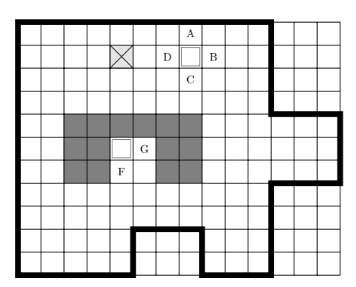
\includegraphics[width=0.5\textwidth]{images/ej5rel1.png}
    \caption{Imagen del mundo bidimensional cuadriculado.}
    \label{fig:mundo}
\end{figure}

\subsubsection*{Solución}

Cálculo de una casilla física (Potencial artificial): 

\begin{itemize}
    \item Componente atractica:
    $p_a(X) = K_1d(X)^2$
    \item Componente repulsica: 
    $p_r(X) = \frac{k_2}{d_0(X)^2}$
\end{itemize}

Aplicando las fórmulas en el ejercicio:

\begin{align*}
    P_a(x) = d(x,obj)^2 \\
    P_r(x) = \frac{1}{d(x,obst)^2} \\
    P(x) = P_a(x)+P_r(x) \\
    P(A) = 4^2 +  \frac{1}{1^2} = 17\\
    P(B) = 4^2 + \frac{1}{2^2} = 16,25\\
    P(C) = 4^2 + \frac{1}{2^2} = 16,25\\
    P(D) = 2^2 + \frac{2^2}{2^2} = 4,25
\end{align*}

Como solución, si debemos de elegir uno en base al potencial nos quedaríamos con D.

Para el 2º apartado:

\begin{align*}
    P(G) = 5^2+ \frac{1}{1^2} = 26 \\
    P(F) = 5^2+ \frac{1}{1^2} = 26
\end{align*}

En este caso al haber empate da igual cual cogemos.

\begin{align}
    P(\text{casilla marcada}) = 4^2 + \frac{1}{1^2} = 17
\end{align}

La casilla del cuadrado es la que menos potencial tiene por lo que debemos de quedarnos con esa (Ecuación 1.1).




% \chapter{Búsqueda en Espacios de Estados}
% \section{Apuntes de CLase}
% \subsection{Diseño de un agente deliberativo: búsqueda en espacios de estados}

El agente dispone de un modelo del mundo donde actúa, modelo de efectos de las acciones sobre el mundo, es capaz de razonar sobre esos modelos para decidir que hacer para conseguir un objetivo.


Tras esta introducción, vamos a pasar a ver el espacio de estados.

\textbf{Espacio de Estados: } Representación del
conocimiento a través de las acciones del
agente.

\textbf{Búsqueda en Espacios de Estados: } Resolución del problema mediante proyección
de las distintas acciones.

Como ejemplo de agente deliberativo, se trata \textit{el problema del viajante de comercio}.



\newpage
% Referencias
\begin{thebibliography}{99}
\bibitem{Referencia1}
Ismael Sallami Moreno, \textbf{Estudiante del Doble Grado en Ingeniería Informática + ADE}, Universidad de Granada, 2025.
% \bibitem{Referencia2}
% Autor(es), \emph{Título del libro}, Editorial, año.

% \bibitem{Referencia3}
% Autor(es), \emph{Título del documento}, Nombre de la Conferencia, páginas, año.
\end{thebibliography}

\end{document}
